% =====================================================================
%  Rozdział 5 - wersja robocza do przeredagowania
%  Dane: wyniki/E4 (22-24.10.2026, powtórka Argon2 1 GiB 8.11.2026)
%  Wszystkie liczby zweryfikowane z plików podsumowań w repozytorium.
%  Wykresy: tools/wykresy-praca.py r5
% =====================================================================
\chapter{Badanie wydajności kryptoanalizy offline z~wykorzystaniem GPU}\label{ch:gpu}

W rozdziale przedstawiono pomiary szybkości, z~jaką konsumencka karta graficzna sprawdza kandydatów na hasło chroniące zaszyfrowane pliki. Rozważany jest atak offline, w~którym napastnik dysponuje kopią pliku i~sprawdza kolejne hasła bez ograniczeń narzucanych przez usługę sieciową. Jedyną przeszkodą jest wtedy koszt obliczeniowy funkcji wyprowadzania klucza z~hasła (ang. \ang{key derivation function}, KDF), omówionej w~podrozdziale~\ref{sec:kdf}. Celem pomiarów było wyznaczenie tego kosztu dla funkcji różnego typu, zbadanie jego zależności od parametrów oraz sprawdzenie, czy funkcje wymagające dużej ilości pamięci (ang. \ang{memory-hard}) rzeczywiście ograniczają przewagę karty graficznej nad procesorem. Pomiary mierzą wyłącznie przepustowość sprawdzania kandydatów; nie dotyczą odtworzenia żadnego rzeczywistego hasła, a~ich wynikiem jest koszt, jaki zabezpieczenie narzuca atakującemu.

% ---------------------------------------------------------------------
\section{Zakres i~plan eksperymentu}\label{sec:gpu-plan}

Pomiary wykonano na platformie opisanej w~podrozdziale~\ref{sec:platforma}: karta NVIDIA GeForce GTX~1660 (6~GB), procesor AMD Ryzen~5~5600, program Hashcat 7.1.2. Maszyny wirtualne laboratorium pozostawały w~tym czasie wyłączone, aby nie obciążały platformy. Zaplanowano cztery serie pomiarów (tabela~\ref{tab:r5-pomiary}).

\begin{table}[htbp]
\centering\small
\begin{tabularx}{\textwidth}{@{}c >{\raggedright\arraybackslash}p{3.5cm} L c c@{}}
\toprule
\textbf{Seria} & \textbf{Zakres} & \textbf{Sposób pomiaru} & \textbf{Powt.} & \textbf{Data} \\
\midrule
1 & 6~formatów, GPU & wbudowany test wydajności (\kod{-b}) na wzorcowych próbkach & 3 + 3 & 22, 23.10 \\
2 & własne pliki, GPU & pomiar przepustowości przez 40~s: VeraCrypt z~trzema wartościami PIM, 7-Zip, KeePass AES-KDF & 3 & 24.10 \\
3 & 5~formatów, GPU i~CPU & test \kod{-b} osobno na obu urządzeniach & 2 & 24.10 \\
4 & Argon2id 64, 256, 1024~MiB; GPU i~CPU & pomiar przepustowości przez 40--60~s & 2 / 3 & 24.10, 8.11 \\
\bottomrule
\end{tabularx}
\caption{Serie pomiarów wydajności kryptoanalizy}
\label{tab:r5-pomiary}
\end{table}

Pliki testowe utworzono tak, aby dwa pliki tego samego rodzaju różniły się tylko jednym parametrem (tabela~\ref{tab:r5-pliki}). Pozwala to przypisać zmianę wyniku jednej przyczynie. Bazy KeePass w~formacie KDBX~4 z~funkcją Argon2 przygotowano, ale nie udało się ich użyć: narzędzie wyodrębniające materiał do analizy obsługuje jedynie starszy format KDBX~3.1 i~dla formatu KDBX~4 zgłaszało błąd nieznanej wersji. Z~tego powodu wpływ pamięci funkcji Argon2 zbadano w~serii~4 na skrótach Argon2id wygenerowanych biblioteką \kod{argon2-cffi}, różniących się wyłącznie parametrem pamięci, przy stałych parametrach czasu $t = 3$ i~równoległości $p = 1$. Zestaw ten odpowiada drugiemu z~wariantów zalecanych w~RFC~9106~\cite{rfc9106}.

\begin{table}[htbp]
\centering\small
\begin{tabularx}{\textwidth}{@{}>{\raggedright\arraybackslash}p{3.1cm} >{\raggedright\arraybackslash}p{3.1cm} L@{}}
\toprule
\textbf{Plik} & \textbf{Funkcja KDF} & \textbf{Parametr kosztu} \\
\midrule
3~kontenery VeraCrypt (AES) & PBKDF2-HMAC-SHA-512 & PIM 1 / 250 / 500, tj. 16\,000 / 265\,000 / 515\,000 iteracji \\
archiwum 7-Zip (AES-256) & SHA-256 iterowane & $2^{19}$ iteracji, z~weryfikacją danych archiwum \\
baza KeePass KDBX~3.1 (AES) & AES-KDF & 100\,000 rund \\
3~bazy KeePass KDBX~4 (AES) & Argon2d & 64 / 256 / 1024~MiB (nieużyte) \\
3~skróty Argon2id & Argon2id & 64 / 256 / 1024~MiB, $t = 3$, $p = 1$ \\
\bottomrule
\end{tabularx}
\caption{Pliki i~skróty testowe; kolejne pliki tego samego rodzaju różnią się jednym parametrem}
\label{tab:r5-pliki}
\end{table}

Przepustowość mierzono dwiema metodami. W~seriach~1 i~3 użyto wbudowanego testu wydajności programu (\kod{-b}), który podaje liczbę sprawdzeń na sekundę dla skrótu wzorcowego. W~seriach~2 i~4 program sprawdzał kandydatów z~ustalonej przestrzeni przez zadany czas, a~jako wynik przyjęto liczbę kandydatów podzieloną przez czas. W~seriach~2 i~4 nie dążono do odgadnięcia hasła, lecz jedynie do zmierzenia tempa sprawdzania; przestrzeń kandydatów dobrano tak, aby żaden z~nich nie był właściwym hasłem. Każdy pomiar powtarzano (tabela~\ref{tab:r5-pomiary}) i~podawano wartość średnią. Dla funkcji najwolniejszych, gdzie tempo spada do pojedynczych sprawdzeń na sekundę, zaokrąglany odczyt programu jest zbyt zgrubny, więc tempo wyznaczano z~przyrostu licznika postępu między dwoma odczytami stanu.

Aby wykluczyć wpływ nagrzania karty na wyniki, w~czasie części pomiarów rejestrowano co około 2~s jej temperaturę, taktowanie i~pobór mocy. Przebieg dla najdłuższej serii (VeraCrypt, seria~2) przedstawia rysunek~\ref{rys:karta}. Pod pełnym obciążeniem temperatura rdzenia nie przekroczyła 66~$^\circ$C, a~taktowanie rdzeni utrzymywało się w~przedziale 1920--1980~MHz bez tendencji spadkowej. Temperatura pozostawała więc znacznie poniżej progu obniżania taktowania, a~karta nie ograniczała wydajności w~trakcie pomiaru. Rozrzut między powtórzeniami nie przekraczał 1\% dla wszystkich funkcji poza 7-Zip (5,8\%, co wyjaśniono w~podrozdziale~\ref{sec:gpu-compute}), co potwierdza powtarzalność warunków.

\begin{figure}[htbp]
\centering
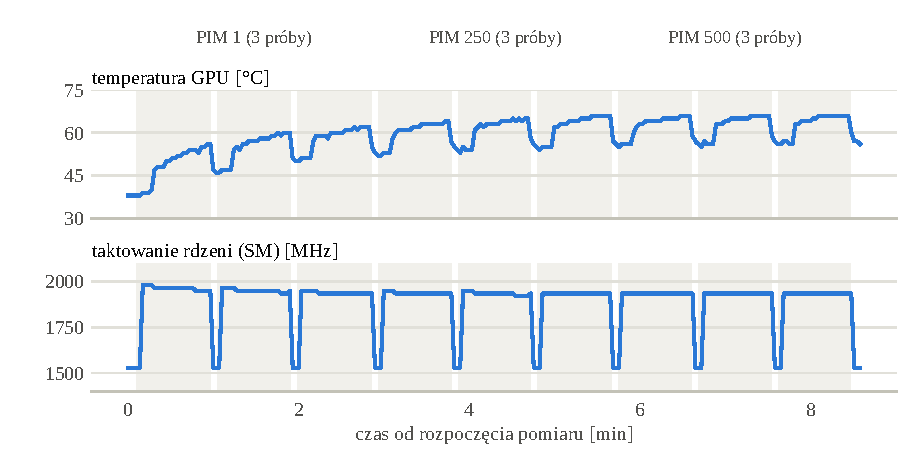
\includegraphics[width=\textwidth]{rysunki/r5-karta.pdf}
\caption{Temperatura i~taktowanie karty w~trakcie serii pomiarów VeraCrypt; szarym tłem oznaczono okresy obciążenia}
\label{rys:karta}
\end{figure}

% ---------------------------------------------------------------------
\section{Wyniki dla algorytmów compute-hard}\label{sec:gpu-compute}

Pierwszą serię pomiarów wykonano wbudowanym testem wydajności dla sześciu formatów, od szybkich funkcji skrótu po funkcje wyprowadzania klucza (tabela~\ref{tab:r5-benchmark}). Różnice sięgają ośmiu rzędów wielkości: szybkie funkcje skrótu MD5 i~NTLM osiągają dziesiątki miliardów sprawdzeń na sekundę, podczas gdy funkcje KDF spowalniają atak od czterech (7-Zip) do ponad siedmiu (Argon2) rzędów wielkości względem MD5. Rozkład prędkości na skali logarytmicznej przedstawia rysunek~\ref{rys:predkosci}. Potwierdza to, że sama szybka funkcja skrótu nie nadaje się do ochrony haseł, a~właściwą barierą dla atakującego jest dopiero funkcja KDF o~odpowiednim koszcie.

\begin{table}[htbp]
\centering\small
\begin{tabular}{@{}llrr@{}}
\toprule
\textbf{Funkcja} & \textbf{Typ} & \textbf{Prędkość GPU [H/s]} & \textbf{Spowolnienie} \\
\midrule
MD5                        & szybka funkcja skrótu & 20\,070\,400\,000 & 1$\times$ \\
NTLM                       & szybka funkcja skrótu & 34\,954\,233\,333 & 0,57$\times$ \\
7-Zip (SHA-256)            & compute-hard & 309\,633 & 64\,820$\times$ \\
KeePass AES-KDF (KDBX~3.1) & compute-hard & 19\,638 & 1\,022\,001$\times$ \\
VeraCrypt (PBKDF2-SHA-512) & compute-hard & 782 & 25\,654\,538$\times$ \\
KeePass Argon2 (KDBX~4)    & memory-hard  & 460 & 43\,599\,710$\times$ \\
\bottomrule
\end{tabular}
\caption{Wbudowany test wydajności: prędkość na GPU i~krotność spowolnienia względem MD5 (wartość poniżej~1 oznacza funkcję szybszą niż MD5)}
\label{tab:r5-benchmark}
\end{table}

\begin{figure}[htbp]
\centering
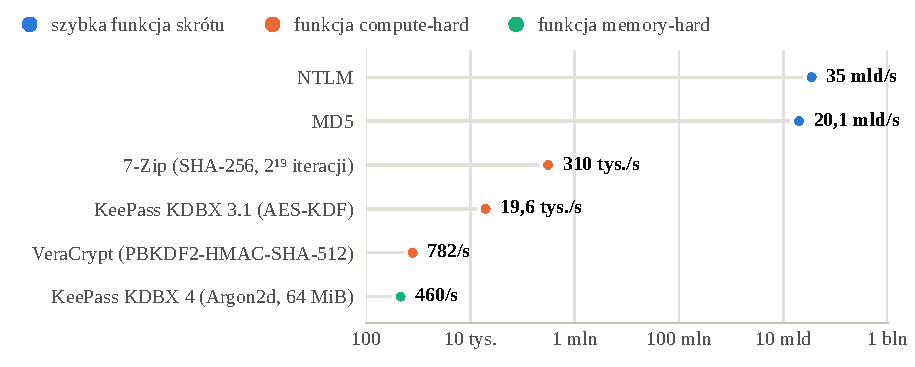
\includegraphics[width=\textwidth]{rysunki/r5-predkosci.pdf}
\caption{Prędkość sprawdzania kandydatów na GPU dla sześciu formatów (skala logarytmiczna)}
\label{rys:predkosci}
\end{figure}

Wbudowany test posługuje się jednak wzorcowymi skrótami o~parametrach dobranych przez autorów narzędzia, które nie muszą odpowiadać plikom spotykanym w~praktyce. Dlatego dwie funkcje compute-hard zmierzono dodatkowo na własnych plikach o~znanych parametrach (tabela~\ref{tab:r5-wlasne}). W~obu przypadkach prędkość okazała się niższa niż w~teście wbudowanym. Dla KeePass AES-KDF stosunek $19\,638 / 4\,734 \approx 4{,}1$ odpowiada liczbie 100\,000~rund w~pliku testowym, większej niż w~skrócie wzorcowym. Dla 7-Zip różnica jest znacznie większa, ponieważ przy rzeczywistym archiwum program musi dla każdego kandydata odszyfrować i~zweryfikować właściwe dane, a~nie tylko sprawdzić krótki wzorzec; stąd także wyższy rozrzut wyników (5,8\%), zależny od zawartości archiwum. Wynika z~tego, że wbudowany test zawyża prędkość atakującego względem realnych plików z~poprawnie dobranym kosztem, a~rzetelna ocena bezpieczeństwa wymaga pomiaru na plikach o~znanych parametrach.

\begin{table}[htbp]
\centering\small
\begin{tabularx}{\textwidth}{@{}L >{\raggedright\arraybackslash}p{3.4cm} r r r@{}}
\toprule
\textbf{Plik} & \textbf{Parametr kosztu} & \textbf{GPU [H/s]} & \textbf{Rozrzut} & \textbf{Test \kod{-b} [H/s]} \\
\midrule
archiwum 7-Zip (AES-256) & $2^{19}$ iteracji SHA-256, weryfikacja danych & 6\,735 & 5,8\% & 309\,633 \\
baza KeePass AES-KDF (KDBX~3.1) & 100\,000 rund & 4\,734 & 0,5\% & 19\,638 \\
\bottomrule
\end{tabularx}
\caption{Pomiar na własnych plikach compute-hard w~zestawieniu z~testem wbudowanym}
\label{tab:r5-wlasne}
\end{table}

% ---------------------------------------------------------------------
\section{Wpływ parametrów kosztu na wydajność}\label{sec:gpu-koszt}

Funkcje compute-hard pozwalają dobrać koszt ataku przez liczbę iteracji. Zależność tę zmierzono na trzech kontenerach VeraCrypt różniących się wyłącznie parametrem PIM, który steruje liczbą iteracji PBKDF2 według wzoru $15\,000 + \text{PIM} \times 1\,000$. Wyniki zawiera tabela~\ref{tab:r5-pim}, a~ich przebieg -- rysunek~\ref{rys:pim}.

\begin{table}[htbp]
\centering\small
\begin{tabular}{@{}rrrrr@{}}
\toprule
\textbf{PIM} & \textbf{Iteracje} & \textbf{Prędkość [H/s]} & \textbf{Rozrzut} & \textbf{Prędkość $\times$ iteracje} \\
\midrule
1   & 16\,000  & 20\,590,7 & 0,6\% & 329,5~mln \\
250 & 265\,000 & 1\,278,3  & 0,0\% & 338,7~mln \\
500 & 515\,000 & 659,0     & 0,0\% & 339,4~mln \\
\bottomrule
\end{tabular}
\caption{VeraCrypt: wpływ liczby iteracji PBKDF2 (parametr PIM) na prędkość ataku}
\label{tab:r5-pim}
\end{table}

\begin{figure}[htbp]
\centering
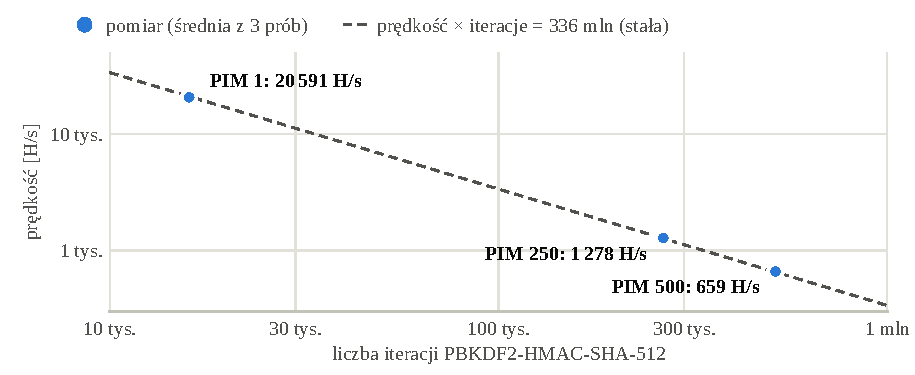
\includegraphics[width=\textwidth]{rysunki/r5-pim.pdf}
\caption{VeraCrypt: prędkość ataku w~funkcji liczby iteracji (skala logarytmiczna na obu osiach)}
\label{rys:pim}
\end{figure}

Prędkość jest odwrotnie proporcjonalna do liczby iteracji: iloczyn prędkości i~liczby iteracji pozostaje niemal stały (329--339~mln), a~przy 32-krotnym wzroście liczby iteracji (z~16\,000 do~515\,000) prędkość spada około 31-krotnie (z~20\,591 do~659~H/s). Parametr kosztu przekłada się więc niemal liniowo na nakład pracy atakującego, co pozwala obrońcy dobrać go do dostępnej mocy obliczeniowej przeciwnika. Nieco niższy iloczyn dla PIM~1 wynika ze stałego narzutu na każdego kandydata (uruchomienie jądra obliczeniowego, odczyt kontenera), który przy małej liczbie iteracji waży proporcjonalnie więcej. Wartość tę wykorzystano też do wyznaczenia odniesienia na rysunku~\ref{rys:pim} (linia stałego iloczynu, średnio 336~mln).

Ograniczeniem funkcji compute-hard jest to, że koszt jednego sprawdzenia rośnie tak samo dla obrońcy, jak i~dla atakującego, a~atakujący dysponuje zwykle znacznie wydajniejszym sprzętem. Skala tej przewagi sprzętowej jest przedmiotem podrozdziału~\ref{sec:gpu-cpu}.

% ---------------------------------------------------------------------
\section{Wyniki dla algorytmów memory-hard}\label{sec:gpu-memory}

Funkcje memory-hard ograniczają atak w~inny sposób: wymagają, by każde sprawdzenie dysponowało dużym, osobnym blokiem pamięci. Masowa równoległość karty graficznej opiera się na jednoczesnym liczeniu tysięcy kandydatów, a~każdy z~nich potrzebuje wtedy własnego bloku pamięci. Gdy pamięć karty się wyczerpuje, liczba równolegle sprawdzanych kandydatów spada, a~wraz z~nią przewaga karty~\cite{eum2023}. Zależność tę zmierzono dla funkcji Argon2id przy trzech rozmiarach pamięci (64, 256 i~1024~MiB) i~stałych pozostałych parametrach, na GPU i~na CPU (tabela~\ref{tab:r5-argon2}, rysunek~\ref{rys:argon2}).

\begin{table}[htbp]
\centering\small
\begin{tabular}{@{}rrrrr@{}}
\toprule
\textbf{Pamięć Argon2} & \textbf{GPU [H/s]} & \textbf{CPU [H/s]} & \textbf{GPU/CPU} & \textbf{Zrównoleglenie GPU} \\
\midrule
64~MiB  & 288,4 & 34,2 & 8,4$\times$ & 83 \\
256~MiB & 30,0  & 7,65 & 3,9$\times$ & 20 \\
1~GiB   & 1,60  & 0,77 & 2,1$\times$ & 4 \\
\bottomrule
\end{tabular}
\caption{Argon2id: prędkość na GPU i~CPU oraz ich stosunek w~funkcji wymaganej pamięci (kolumna ostatnia -- współczynnik zrównoleglenia dobrany przez Hashcat na GPU)}
\label{tab:r5-argon2}
\end{table}

\begin{figure}[htbp]
\centering
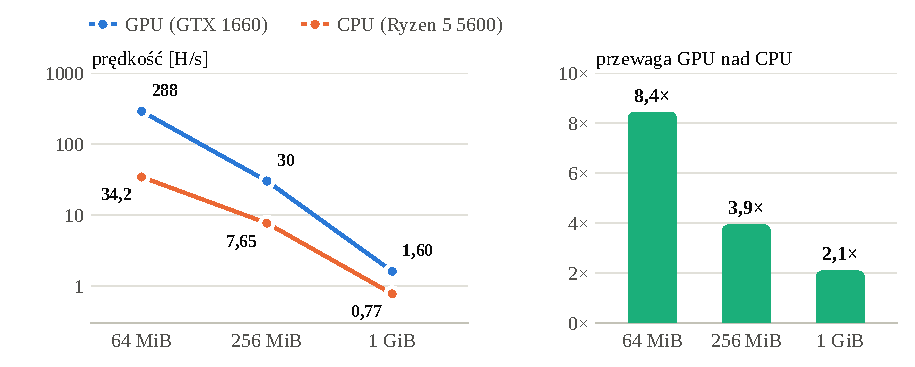
\includegraphics[width=\textwidth]{rysunki/r5-argon2.pdf}
\caption{Argon2id: prędkość na GPU i~CPU (lewy panel) oraz przewaga GPU nad CPU (prawy panel) przy rosnącej pamięci}
\label{rys:argon2}
\end{figure}

Wraz ze wzrostem wymaganej pamięci przewaga GPU nad CPU maleje: z~8,4-krotnej przy 64~MiB, przez 3,9-krotną przy 256~MiB, do 2,1-krotnej przy 1~GiB. Jednocześnie współczynnik zrównoleglenia dobierany przez program na karcie spada z~83 do~4, a~jego iloczyn z~pamięcią pojedynczego sprawdzenia pozostaje rzędu pojemności karty (odpowiednio około 5,2, 5,0 i~4,0~GiB wobec 6~GB karty). Wskazuje to, że liczbę jednocześnie sprawdzanych kandydatów ogranicza nie moc obliczeniowa, lecz pamięć karty -- co jest istotą ochrony, jaką funkcje memory-hard dają przeciwko atakom z~użyciem GPU.

Pomiar dla 1~GiB wykonano jako osobną powtórkę (8.11.2026). We wcześniejszej serii (24.10) przy tym rozmiarze pamięci program kończył się na karcie błędem przydziału bufora i~obliczeń nie wykonywał, podczas gdy powtórka trzykrotnie zakończyła się powodzeniem z~jednakowym wynikiem (rysunek~\ref{rys:argon2-1gib}). Rozbieżność tę przypisano stanowi pamięci karty w~chwili doboru rozmiaru buforów: 1~GiB na pojedyncze sprawdzenie leży na granicy możliwości tej karty, powyżej której przydział bufora bywa odrzucany. W~powtórce program zgłosił ponadto zajęcie około 1,1~GB pamięci karty przez inne procesy i~ograniczył wykorzystanie do 83\%, dlatego zmierzoną prędkość GPU dla 1~GiB należy traktować jako dolne oszacowanie; bez tego ograniczenia stosunek GPU/CPU nie przekroczyłby około 2,5-krotności, co nie zmienia wniosku o~malejącej przewadze karty.

\begin{figure}[htbp]
\centering
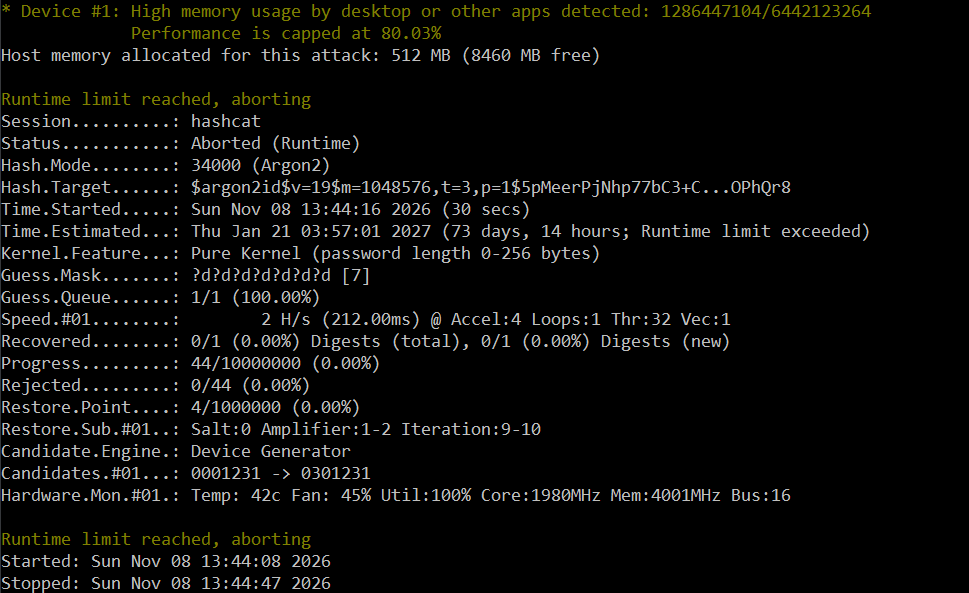
\includegraphics[width=0.85\textwidth]{rysunki/r5-argon2-1gib.png}
\caption{Pomiar Argon2id z~pamięcią 1~GiB na GPU z~widocznym ograniczeniem wykorzystania karty}
\label{rys:argon2-1gib}
\end{figure}

% ---------------------------------------------------------------------
\section{Porównanie GPU i~CPU oraz interpretacja wyników}\label{sec:gpu-cpu}

Przewagę karty graficznej nad procesorem zmierzono osobno dla pięciu funkcji, uruchamiając ten sam test na GPU i~na CPU (tabela~\ref{tab:r5-gpucpu}). Zestawienie wszystkich wyznaczonych stosunków, łącznie z~serią Argon2 z~podrozdziału~\ref{sec:gpu-memory}, przedstawia rysunek~\ref{rys:gpu-cpu}.

\begin{table}[htbp]
\centering\small
\begin{tabular}{@{}lrrr@{}}
\toprule
\textbf{Funkcja} & \textbf{GPU [H/s]} & \textbf{CPU [H/s]} & \textbf{GPU/CPU} \\
\midrule
MD5                         & 20\,016\,200\,000 & 1\,218\,600\,000 & 16,4$\times$ \\
7-Zip (SHA-256)             & 310\,100 & 7\,478 & 41,5$\times$ \\
KeePass AES-KDF             & 19\,794  & 2\,666,5 & 7,4$\times$ \\
VeraCrypt (PBKDF2-SHA-512)  & 786 & 70 & 11,2$\times$ \\
KeePass Argon2 (64~MiB, próbka) & 461 & 36 & 12,8$\times$ \\
\bottomrule
\end{tabular}
\caption{Przewaga GPU nad CPU dla pięciu funkcji (test wbudowany)}
\label{tab:r5-gpucpu}
\end{table}

\begin{figure}[htbp]
\centering
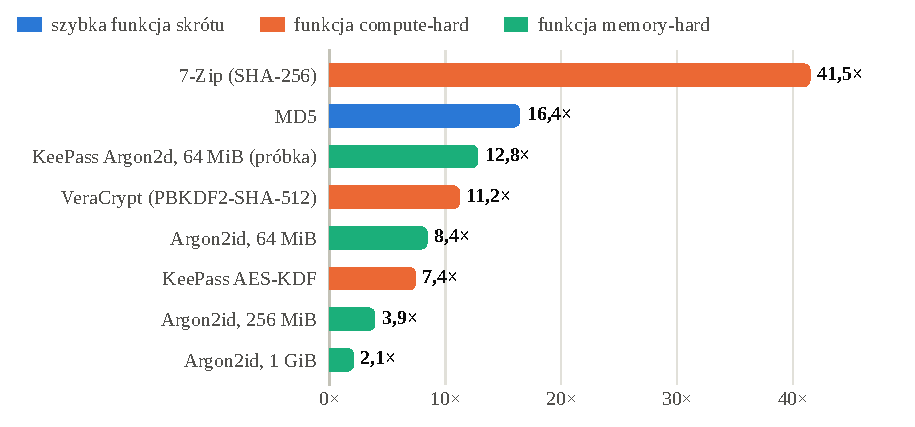
\includegraphics[width=\textwidth]{rysunki/r5-gpu-cpu.pdf}
\caption{Przewaga GPU nad CPU dla wszystkich badanych funkcji, uporządkowana malejąco}
\label{rys:gpu-cpu}
\end{figure}

Przewaga GPU nie zależy wprost od podziału na funkcje compute-hard i~memory-hard, lecz od tego, jak dana funkcja odwzorowuje się na sprzęt:
\begin{itemize}
  \item \textbf{7-Zip daje najwyższą przewagę (41,5$\times$)}, ponieważ opiera się na funkcji SHA-256 wykonującej działania 32-bitowe, w~których procesory graficzne są szczególnie wydajne.
  \item \textbf{KeePass AES-KDF daje najniższą przewagę (7,4$\times$)}, ponieważ procesor Ryzen~5~5600 ma sprzętowe wsparcie szyfrowania AES (zestaw instrukcji AES-NI) i~wykonuje rundy AES bardzo wydajnie, przez co dystans do karty maleje.
  \item \textbf{VeraCrypt (11,2$\times$)} korzysta z~PBKDF2-HMAC-SHA-512, czyli działań 64-bitowych, mniej korzystnych dla konsumenckiej karty, więc procesor relatywnie nadrabia.
  \item \textbf{Argon2 przy 64~MiB daje jeszcze 8,4--12,8$\times$} na korzyść GPU, ponieważ przy tej ilości pamięci karta mieści wiele równoległych sprawdzeń; dopiero większa pamięć ujawnia własność memory-hard (podrozdział~\ref{sec:gpu-memory}). Różnica między wartością 12,8$\times$ z~próbki wbudowanej a~8,4$\times$ z~własnego skrótu wynika z~innych parametrów czasu ($t = 2$ wobec $t = 3$); porównywalny jest trend, nie wartości bezwzględne.
\end{itemize}

Wynika z~tego, że sama klasyfikacja funkcji jako memory-hard nie gwarantuje najmniejszej przewagi GPU przy niskich parametrach pamięci. Najskuteczniej ogranicza tę przewagę albo funkcja oparta na działaniach sprzętowo przyspieszanych w~procesorze (AES-KDF), albo -- co pokazała seria~4 -- funkcja memory-hard z~odpowiednio dużą pamięcią. Z~punktu widzenia obrońcy najpewniejszą ochroną jest funkcja memory-hard z~parametrem pamięci przekraczającym możliwości taniego sprzętu masowo równoległego: przy 1~GiB przewaga karty spadła do około dwukrotności, a~bezwzględna prędkość ataku -- do pojedynczych sprawdzeń na sekundę. Jest to ilościowe potwierdzenie zaleceń doboru funkcji wyprowadzania klucza, przyjętych w~warstwie ochrony danych opisanej w~rozdziale~\ref{ch:obrona}.
